\section{Model design}
\label{Design}
The game was modeled using different designs. This section will discuss the designs and their up- and down-sides.
The characteristics of GROOVE should be taken into account to optimize the simulation performance. 
In each design the following properties were used:

\begin{itemize}
\item The type "Game" is used to model the the game itself.
\item A type "Player" is used to model a player of the game. The game node features an "currentPlayer" edge to the player whoms turn it is.
\item A type "Space" is used to model a space on the board where a marble can be placed. A marble placement of a player on a space is defined as an "marble" edge from the player node to the space node.
\item An edge "currentPlayer", from the Game to a Player, models whose turn it is.
\item "nextPlayer" Edges between Player nodes indicate the order in which the Players have to play.
\item A "marble" edge from a Player to a Space indicates that a Player has placed a marble on that Space.
\end{itemize}

Also the following rule names were used:

\begin{itemize}
\item "placeMarble": A rule in which the currentPlayer can place a marble on the board.
\item "rotateClockwise" and "rotateCounterClockwise": The rules that model the rotation of a Block on the board.
\item "nextPlayer": The rule that provides the turn-taking mechanism of the palers. The turn taking mechanism has been defined as a graph transformation.
When a player has finished its turn, the currentPlayer edge from the game node is shifted to the player which is connected to by the nextPlayer edge.
The global graph transformation defined for the turn taking mechanism is displayed in figure \ref{fig:turn}.
\end{itemize}

\begin{figure}[!h]
    \centering
    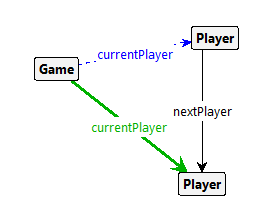
\includegraphics[scale=0.5,clip]{Images/turn.png}
    \caption{Taking turns}
    \label{fig:turn}
\end{figure}

To enforce that the game is played by the rules, a control program has been defined which contains the game flow.
The control program defines the following game flow: As long as possible, a player places a marble, rotates a sub-board and gives the turn to the next player.
The game is finished when a win condition is met, or no marbles can be placed anymore.

\subsection{PentagoXY}
\label{pentagoxy}

The first design modeled the layout of the board by using $x$ and $y$ coordinates for the Spaces where a marble can be placed. 
The board is dynamically generated. The attribute "blocks" determines the size of the board. It indicates the number of blocks in the $x$ and the $y$ direction, with each block being $3*3$ Spaces.
In the start graph there is only one Space node with the coordinates $(0,0)$. Rules were created to create new Spaces in the $x$ and $y$ direction.

A Block on the $x,y$ grid could be identified by the middle Space in the block. Where $x\mod3==1$ and $y\mod3==1$.
Rotating the block was done by changing the coordinate attributes of the Spaces surrounding the middle Space.

\vspace{6pt}

To model the situation where a Player has won, the Direction type was introduced. The Direction node has a $dx$ and a $dy$ attribute.
This way the direction horizontal ($dx=1,dy=0$), vertical ($dx=0,dy=1$) and both diagonal ($dx=1,dy=1$ and $dx=1,dy=-1$) were modeled. 
In the "winner" rule 5 Spaces have to have a marble of the same Player and be spaced repectively $0,1,2,3,4$ times $dx$ and $dy$ for a specific direction.

\vspace{6pt}

This model relies more on attributes than on a graph structure.
The matching strategy of Groove proved to be very inefficient to find a matching for a block. The 9 Space nodes have to be identified by the attributes of the middle space in the block, and the positions relative to these coordinates.
Possible optimizations could be to add flags to the middle space of a Block, and use them to steer the matching strategy of Groove. E.g. to add a flag to the middle Space of the blocks, such that Groove would first try to find these Spaces, instead of trying to find matches for all possible combinations of Spaces.
However it is also possible to add more structure to the graph. 
The extra structure in the model could even convey the intention of the model better to the user, and it might also have better performance in the Groove tool. Therefore a new model of the game was created.

\subsection{PentagoGenerator and Pentago}
\label{pentagoGenerator_and_pentago}

For the second iteration in the development of the model two production systems were created. The "pentagoGenerator" system to generate the board on which to play, and "pentago" to model the actual rules of the game.

\vspace{6pt}

In "pentagoGenerator" a new type named Block is added. This models a $3*3$ block and makes it easier for Groove to match rules to rotate blocks.
The starting graph again consist of a Game node, nodes for the Players and one Block node. From the Game node the first Player is pointed to by the "currentPlayer" edge, and the players are connected by "nextPlayer" edges that model the order in which they can play.
The Game node again has the attribute "blocks", which defines how many blocks the game board has in the $x$ and $y$ direction.

\vspace{6pt}

With the rules "createBlockX" and createBlockY" new Block nodes are created in the respective direction.
With the rule "createBlock" the 9 Spaces of the actual block are created. Again each Space gets an $x$ and $y$ coordinate appointed to it, calculated using the coordinates of the block and the offsets of the spaces within the block.
Within the block are edges that define how "marble" edges need to move when a block is rotated clockwise (cw) or counter-clockwise (ccw).
An entire block including its spaces is visualized in figure  \ref{fig:p2-block}.

\begin{figure}[!h]
    \centering
    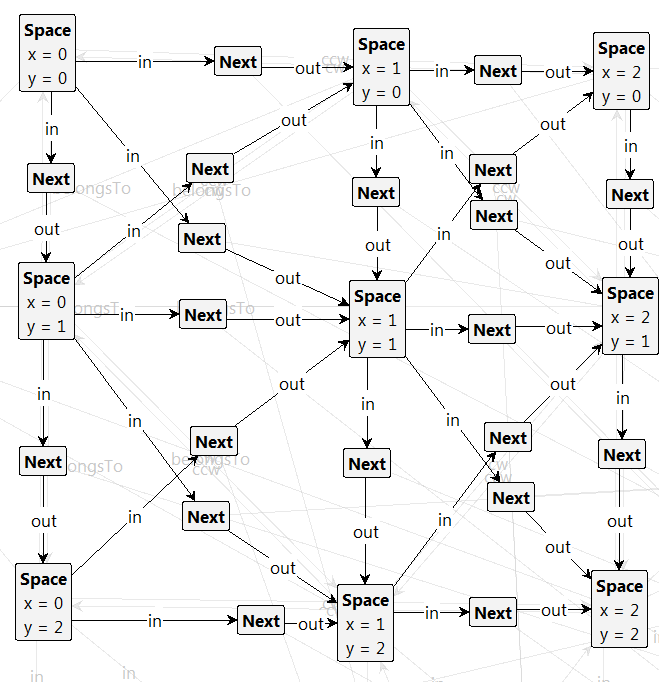
\includegraphics[scale=0.25,clip]{Images/oneblockwithoutbelongs.PNG}
    \caption{A block (sub-board)}
    \label{fig:p2-block}
\end{figure}

\vspace{6pt}

Having 5 marbles in a row is a property that always extends beyond one block.
Therefore the rule "setDirections" is used to dynamically create the structure to model in which directions 5-in-a-row can occur within a block and cross into adjacent blocks.
Again there are 4 Direction nodes in the start graph to represent the directions horizontal ($dx=1,dy=0$), vertical ($dx=0,dy=1$), and both diagonals ($dx=1,dy=1$ and $dx=1,dy=-1$). 
The connection between two spaces is modeled by a Next node that has one "in" edge from the first Space to the Next node, one "out" edge from the Next to the second Space node and a "dir" edge from the Next to the Direction node. This allows to abstract away from the direction in the actual rule to match 5-in-a-row. The connection between two spaces by making use of a direction node is visualized in figure \ref{fig:cspaces}.

\begin{figure}[!h]
    \centering
    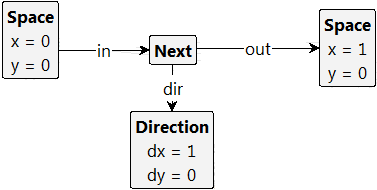
\includegraphics[scale=0.25,clip]{Images/TwoSpacesConnected.PNG}
    \caption{Connected spaces}
    \label{fig:cspaces}
\end{figure}

\vspace{6pt}

In the pentago production system are the rules for the actual game.
It again has the rule "placeMarble" in which the current player can place a marble on the board.

Rotating a block is now done by matching a Block node, and moving all marble edges, from all Players from Spaces that belong to that block, to Spaces that are connected with the direction edge (cw or ccw). The rotation mechanism is visualized in figure \ref{fig:rsb}.

\begin{figure}[!h]
    \centering
    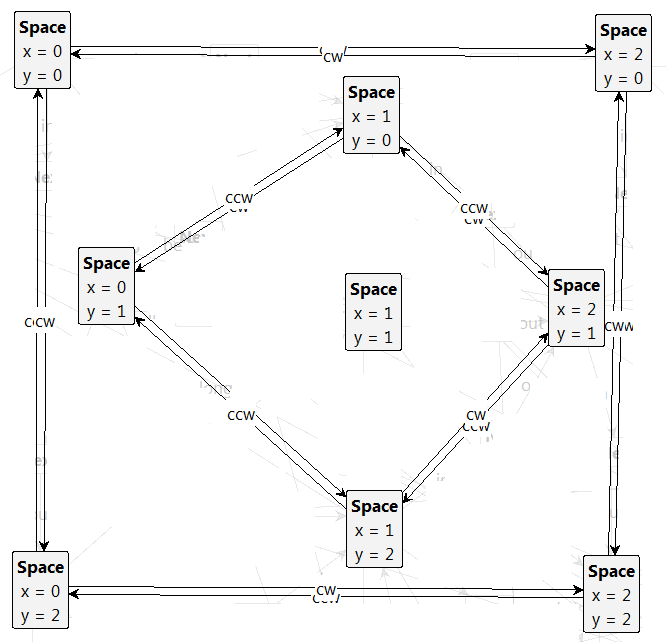
\includegraphics[scale=0.25,clip]{Images/blockforrotation.PNG}
    \caption{Rotating a sub-board}
    \label{fig:rsb}
\end{figure}
\vspace{6pt}

Matching 5-in-a-row is done in the "winner" rule by a rule that matches a Player who has marbles on 5 Spaces that are connected by "in" and "out" edges via Next nodes that are connected to the same Direction node.

In simulation the performance has significantly improved. Rotating blocks is nearly instantaneous. 
However trying to find a match for the "winner" rule takes significant time. 
Finding 5 Spaces out of 36, 4 Next nodes out of 110, 1 Block out of 4 and 1 Player out of 2 with the right connections takes a lot of time if the strategy is not perfect.

\vspace{6pt}

There is more structure in the pentago model than in the pentagoXY model. Dynamically creating the board gives greater flexibility in extending to a multi-player game.
The addition of the Block node nicely captures the notion of the $3*3$ blocks of the game. And as a bonus it also made it a lot better to analyze with Groove.
Using the Next type to abstract away from the directions made it possible to nicely capture the notion of 5-in-a-row for the "winner" rule. However the added complexity in the model also proved to be a bottleneck in analyzing the system.

\subsection{PenagoFinal}

\begin{figure}[!h]
    \centering
    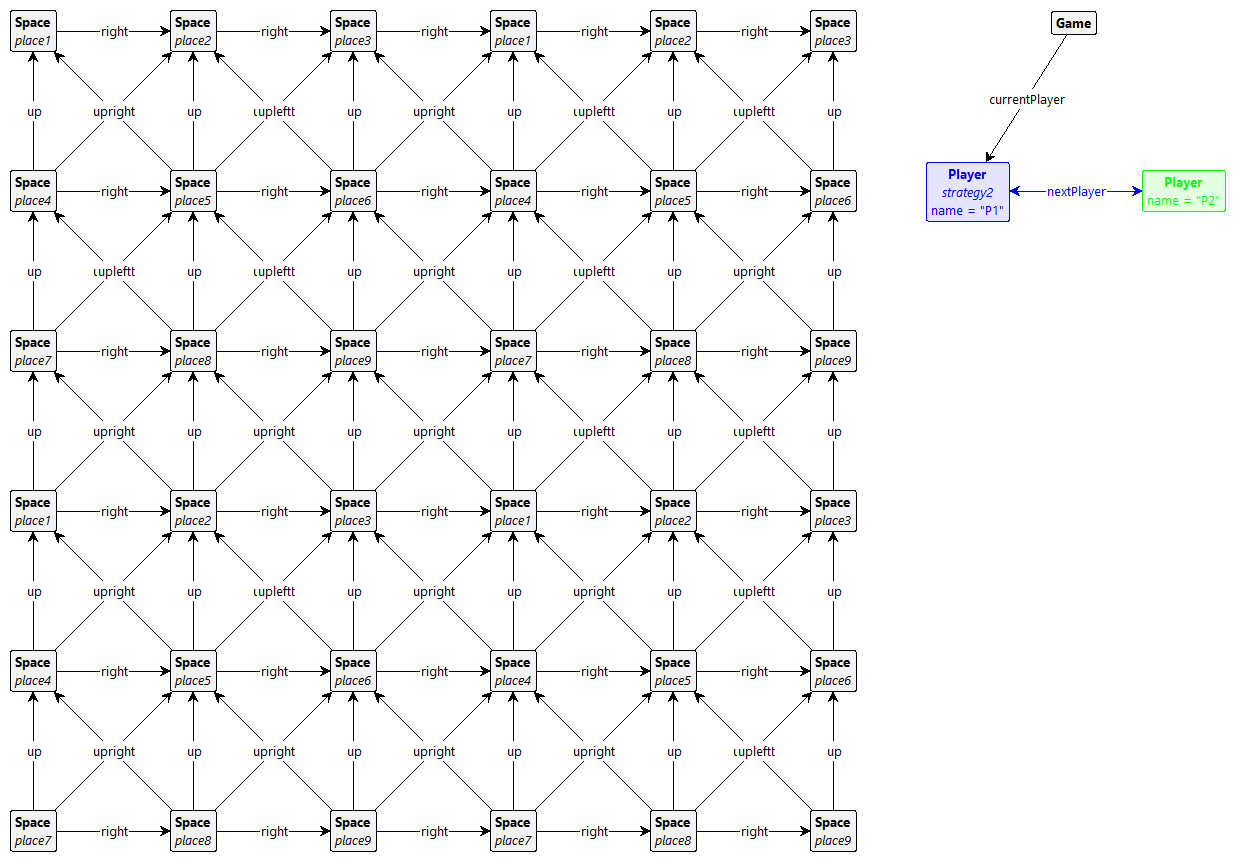
\includegraphics[scale=0.35,clip]{Images/board1.png}
    \caption{Board layout}
    \label{fig:board1}
\end{figure}

This design features 36 spaces in which nodes are connected to their neighbours by horizontal, vertical and diagonal edges.
All spaces in a sub-board hold an unique identifier flag.
The board model is displayed in figure \ref{fig:board1}.

\vspace{6pt}

In this model, the \textit{Game} holds multiple \textit{Players}, which are able to hold multiple \textit{marble} edges to \textit{Spaces}. When the game ends, an edge is created from the \textit{Game} node to a newly created \textit{Finished} node. The full type graph of this model is defined in figure \ref{fig:type_graph_pure_graph}.

\begin{figure}[!h]
    \centering
    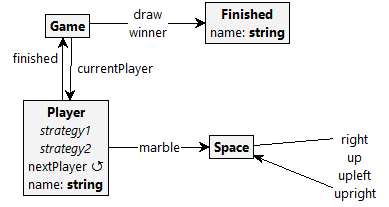
\includegraphics[scale=0.5,clip]{Images/typegraph_puregraphmodel.png}
    \caption{Type graph}
    \label{fig:type_graph_pure_graph}
\end{figure}

\vspace{6pt}

The rotation step in the game flow can be seen as a graph transformation.
In the corresponding graph transformation, the \textit{marble} edges to the nodes on the sub-board are relocated to a clockwise or counter-clockwise node.
This way the board including its connecting edges stay intact.
The graph transformations defined for the rotations are displayed in figure \ref{fig:rotate1}.

\begin{figure}[!h]
    \centering
    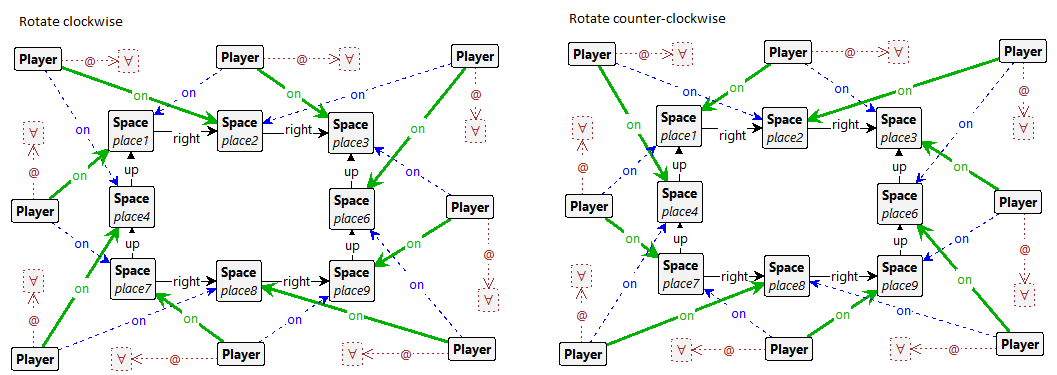
\includegraphics[scale=0.5,clip]{Images/rotate1.png}
    \caption{Rotating a sub-board}
    \label{fig:rotate1}
\end{figure}

\vspace{6pt}

The end-game of pentago is either one player winning the game, or the game ending in a draw.
For a player to win, the player needs to hold \textit{marble} edges to five consecutive nodes.
The game results in a draw when multiple players hold five consecutive nodes simultaniously (this is possible after a rotation), or when no marbles can be placed on the board anymore.

\vspace{6pt}

To check for the winner condition, 4 graph conditions are needed which look whether a row of identical marbles (which are connected by either horizontal, vertical or diagonal edges) exist.
The winner rule which checks for a horizontal row is visualized in figure \ref{fig:endgame1}.
The rules which check for vertical or diagonal rows are identical, except that they check for different edge names.
When a winner rule matches, the \textit{Player(s)} on which the condition matches are connected with a \textit{finished} edge to the \textit{Game}.
The first draw scenario, when multiple players hold a row of consecutive marbles, is achieved when multiple \textit{Players} hold \textit{finished} edges to the \textit{Game} simultaneously.
The draw scenario when no marble can be put on the board anymore, has been defined by using the control program.
When either a winner or a draw is detected, a \textit{winner} or \textit{draw} edge is created between the Game and the Finished node. When a winner is detected, its name is added as an attribute to the \textit{Finished} node. The winner and draw graph condition check for the existence of a \textit{winner} or \textit{draw} edge between \textit{Game} and \textit{Finished}. When it exists the game is finished.

\vspace{6pt}

The seperation of the winning conditions should be seen as a trade-off between scalability and performance: while having 4 individual winning conditions decreases the expandability of the game rules, we have chosen to implement it this way because it decreases the complexity of the computations needed when looking for a winner significantly.

\begin{figure}[!h]
    \centering
    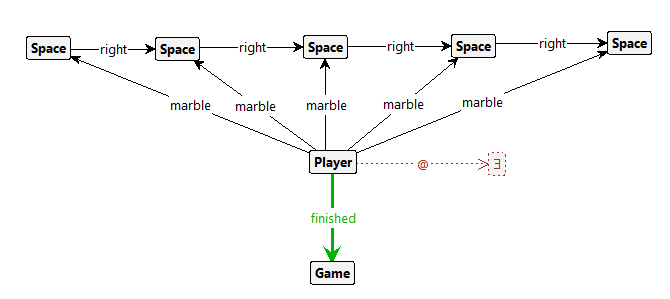
\includegraphics[scale=0.5,clip]{Images/endgame_puregraph.png}
    \caption{Checking for a winner}
    \label{fig:endgame1}
\end{figure}

\vspace{6pt}

While this model is less abstract and thus less scalable than the pentago models described in sections \ref{pentagoGenerator_and_pentago} and \ref{pentagoxy}, the fact that it is a more graph oriented representation makes the model design more clear for users.
Furthermore the usage of edges and node identifiers enable quick matching, which results in a better performance when exploring the state space.
For these reasons this model has been chosen to research smart player strategies.